\documentclass[unknownkeysallowed,table]{beamer}
\usepackage{multimedia}
\usepackage[utf8]{inputenc}
\usepackage{amsthm, amsmath, amssymb}
\usepackage{fourier}
\usefonttheme{professionalfonts}
\usepackage{wasysym}
\usepackage{attrib}
\usepackage{graphicx}
\usepackage{pdfpages}
\usepackage{setspace}
\usepackage{mathtools}
\setbeamersize{text margin left=8mm,text margin right=12mm} 
\usepackage{tikz}
\setbeamerfont*{frametitle}{size=\normalsize,series=\bfseries}
\setbeamercolor{normal text}{fg=black!90}
\usepackage{textcomp}
\usepackage[scaled]{helvet}\renewcommand{\familydefault}{\sfdefault}
\usetikzlibrary{arrows}
\tikzstyle{block}=[draw opacity=0.7,line width=1.4cm]
\usepackage{fancybox}
\newcommand{\ergs}{${\rm erg}\,{\rm s}^{-1}$}
\newcommand{\bfsimb}[1]{\Vec{#1}}
\newcommand{\no}{\nonumber}
\AtBeginSection[]{
  \begin{frame}<beamer>{Table of contents}
    \tableofcontents[currentsection,
    ]
 \end{frame}
}
\setbeamerfont*{frametitle}{size=\normalsize,series=\bfseries}
\usetheme{Singapore}
\setbeamertemplate{navigation symbols}{}
\setbeamertemplate{footline}[frame number]
\setbeamerfont*{frametitle}{size=\normalsize,series=\bfseries}
\title[]{{\small TeV Particle Astrophysics 2025 - València}\vspace{.5cm} \\
\bf{Supernova explosion within an extragalactic jet\\Dynamics and radiative output of such event}}
\author[]{\large \bf{ Bruno Longo} \\
{\scriptsize M. Perucho, V. Bosch-Ramon, J.M. Mart\'i, G. Fichet de Clairfontaine}}

\institute[]{Departament d'Astronomia i Astrof\'isica, Universitat de València }
\titlegraphic{
\includegraphics[width=1cm]{images/uv.png}\hspace{2cm}
\includegraphics[width=4cm]{images/ministero.png}}

\begin{document}
\begin{frame}[plain]
\maketitle
\end{frame}
\section{Within the path of an AGN jet}

\begin{frame}{From jet deceleration to particle acceleration}

		{\scriptsize
	\begin{columns}
		\begin{column}{0.5\textwidth}
			\centering
			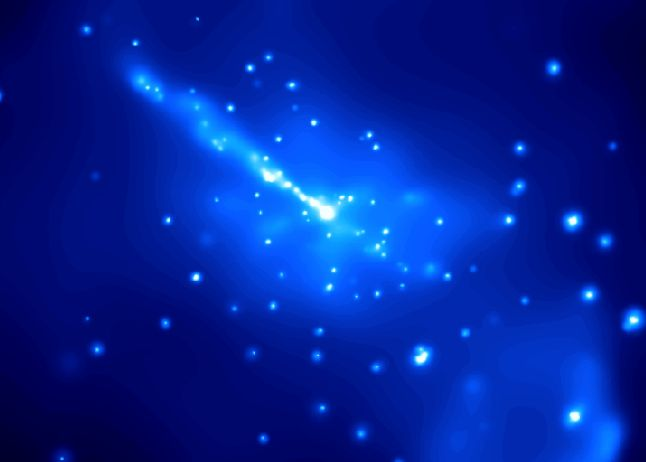
\includegraphics[width=1.1\linewidth]{images/cena_jet.jpg}
			Nearby galaxy Centaurus A in X-ray (Kraft et al 2001, Goodger et al 2010)
				\begin{block}{Entrainment in FRIs}
				Protons or heavier elements (stellar winds, clouds, SN, ambient medium) \\
			    $\rightarrow$ inexorable mass-loading and deceleration
						of the jet (De Young 1986, Bowman et al. 1996)
			\end{block}

		\end{column}
		\begin{column}{0.5\textwidth}
			\centering
			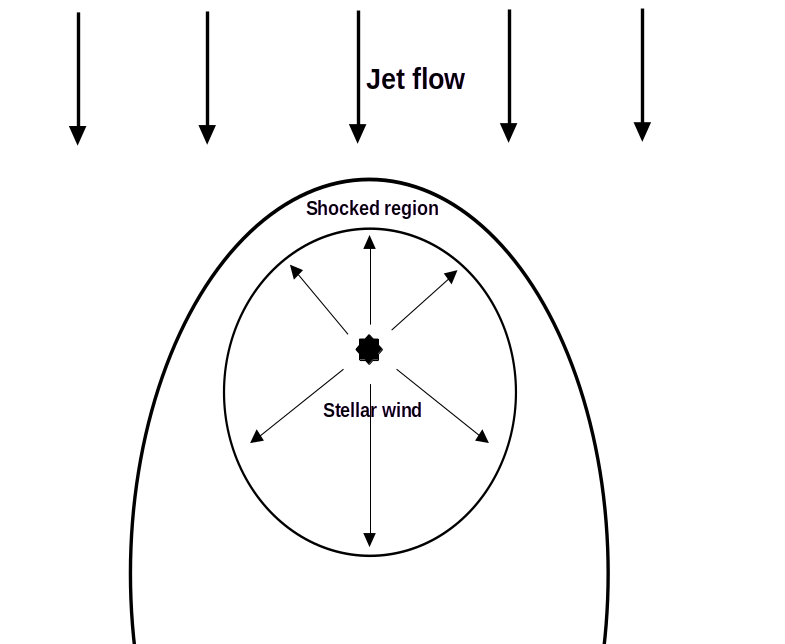
\includegraphics[width=.9\linewidth]{images/jet_wind.png}
				\begin{exampleblock}{Shocks}
				\begin{itemize}
					\item Balance between 2 supersonic matching flows (Komissarov 1994, Hubbard \& Blackman 2006)
					\item Conversion of $E_{k}$ into $U$ \\
						$\rightarrow$ expansion of the shock surface  \\
					\item Acceleration of $e^{-}$, $p$ or heavier ions\\
						$\rightarrow$ possible emissions up to $\gamma$-rays and
						acceleration of UHECR?
				\end{itemize}
			\end{exampleblock}

		\end{column}
	\end{columns}
	}
\end{frame}

\begin{frame}{Jet/star interaction time scale with the distance from the jet base}
	\begin{columns}
		{\scriptsize
		\begin{column}{0.5\textwidth}
			\begin{alertblock}{Close to the AGN | $z<10\,{\rm pc}$}
				\begin{itemize}
					\item Presence of large amounts of gas \\
						$\rightarrow$ lots of stars (RG, MS, AGB..) 
					\item Interaction with the outflow short ($t_{\rm int}=2R_{\rm j}/v_{\rm orb}$, typically 
							$\approx {\rm kyr}$)
								but frequent (short orbital period) (Kurfürst et al. 2024)\\
						$\rightarrow$ small mass loss per interaction  \\
				\end{itemize}
			\end{alertblock}
			\begin{block}{Far from the AGN | $z>{\rm kpc}$}
				\begin{itemize}
					\item The jet has expanded \\
							$\rightarrow$ Jet/star interaction time scale increases
								(typ. $\approx{\rm Myr}$)
					\item Stellar population typ. $\approx 1 {\rm star/pc}^{3}$ \\
						$\Rightarrow$ If SRG, eventual explosion
				\item 70 SN/century and ~0.01\% of them inside the jet (Vieyro et al. 2019)
				\end{itemize}
			\end{block}
		\end{column}
		\begin{column}{0.5\textwidth}
			\centering
			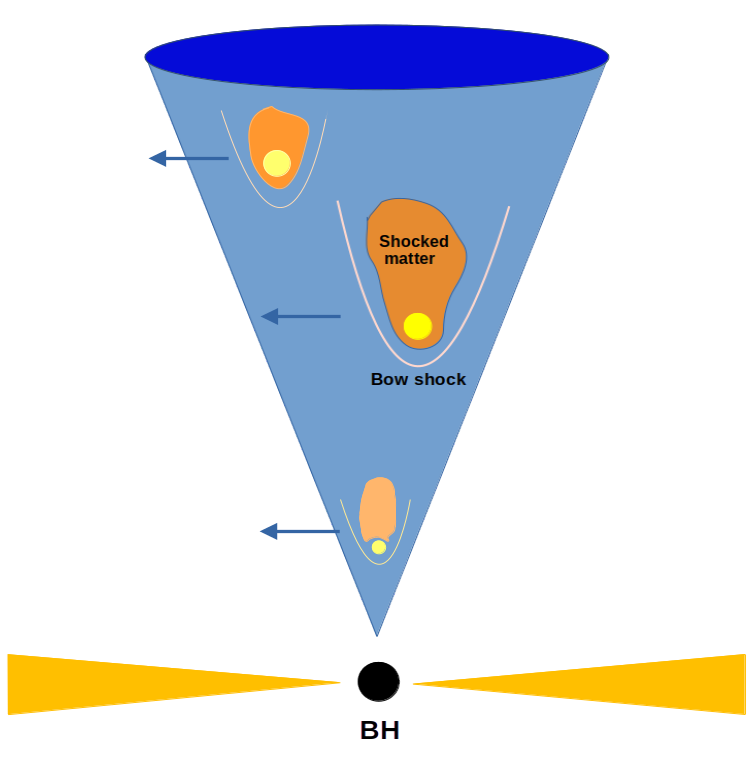
\includegraphics[width=\linewidth]{images/jet_mobstacles.png}
			\bf{A SRG can explode within the jet flow (Bosch-Ramon 2023) \\
		If the jet ram pressure becomes dominant over the SN remnant \\
						$\Rightarrow$ eventual disruption	}

		\end{column}}	
	\end{columns}
\end{frame}

\section{Supernova explosion}

\begin{frame}{3D RHD simulations (Longo et al. 2025)}
	\begin{columns}

		{\footnotesize
		\begin{column}{0.5\textwidth}
		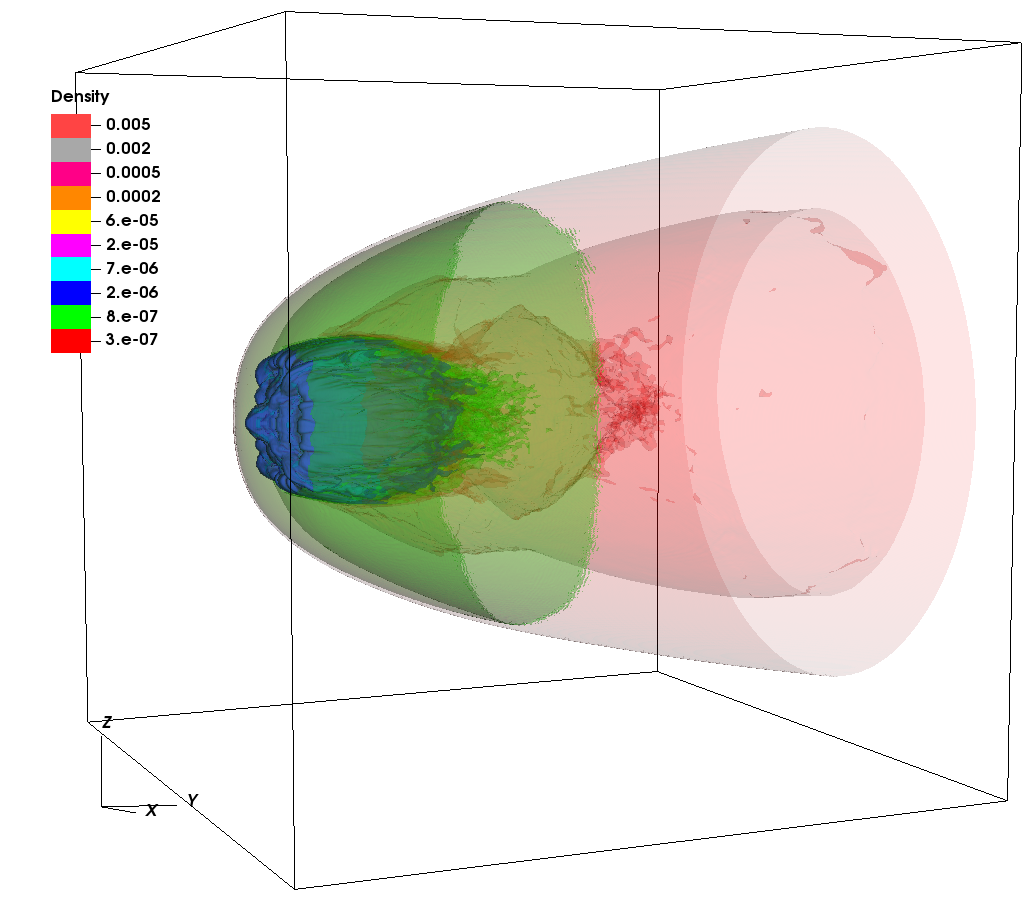
\includegraphics[width=\textwidth]{images/3d_shot_rho.png}
				\vspace{-.5cm}
		 \begin{itemize}
		  \item We start $\approx 10^{3}\,{\rm yr}$ post explosion,
		 				located far from the jet walls
		  \item $R_{\rm j} >> R_{\rm SN}\quad \Rightarrow R_{\rm SN}\approx 10^{-2} R_{\rm j}$ \\
		  \item  Uniform ejecta $\rho_{\rm SN},p_{\rm SN}>>\rho_{\rm j},p_{\rm j}$
		  \item Jet and ejecta: ionized gas of protons and electrons
		 \end{itemize}

		\end{column}}
		\begin{column}{0.7\textwidth}
			{\scriptsize
		 \begin{columns}\begin{column}{.5\textwidth}
		  \begin{alertblock}{Jet properties}
			\begin{itemize}
		      \item $R_{\rm j} = 100\,{\rm pc}$
			  \item $L_{\rm j} = 10^{44}\,{\rm erg}\,{\rm s}^{-1}$
			  \item $\Gamma_{\rm j}=2$
			  \item $h_{\rm j} = 1.1c^{2}$
			  \item $\rho_{\rm j} = 6\cdot10^{-30}\,{\rm g}/{\rm cm}^{3}$
			  \item $T_{\rm j} = 2\times 10^{11} K$
			\end{itemize}
		   \end{alertblock}
		  \end{column}
		  \hspace{-2cm}
		  \begin{column}{.5\textwidth}
		   \begin{exampleblock}{SN properties}
		     \begin{itemize}
					\item $M_{\rm SN}=2\,M_\odot$
					\item $E_{\rm SN}=10^{51}\,{\rm erg}$
					\item $R_{\rm SN}=1.1\,{\rm pc}$
					\item $\rho_{\rm SN}= 2.4\cdot10^{-23}\,{\rm g}/{\rm cm}^{3}$
					\item $T_{\rm SN} = 10^{9}\,K$
					\item $v_{\rm orb} = 200\,{\rm km}\,{\rm s}^{-1}$
				\end{itemize}
			\end{exampleblock}
		 \end{column}
		\end{columns}}
		\vspace{1cm}
		{\scriptsize
		\begin{block}{Code: \texttt{Ratpenat} (Perucho 2010)}
			OpenMPI+OpenMP HRSC 3D RHD code, Marquina 1998 fluxes, PPM recon, Synge equation
			\\
				Conservative form equations $\frac{\partial U}{\partial t}+\frac{F^{i}}{\partial x^{i}}=0$\\
				Where $U=(D,S^{j},\tau)^{T}$ and $F = (Dv^{i}, S^{j}v^{i}+p\delta^{ij}, S^{i}-Dv^{i}) $
		\end{block}
			}
		\end{column}
	\end{columns}
\end{frame}
\begin{frame}{2D cuts through the 3D physical domain}
\begin{columns}
	\begin{column}{.9\textwidth}
	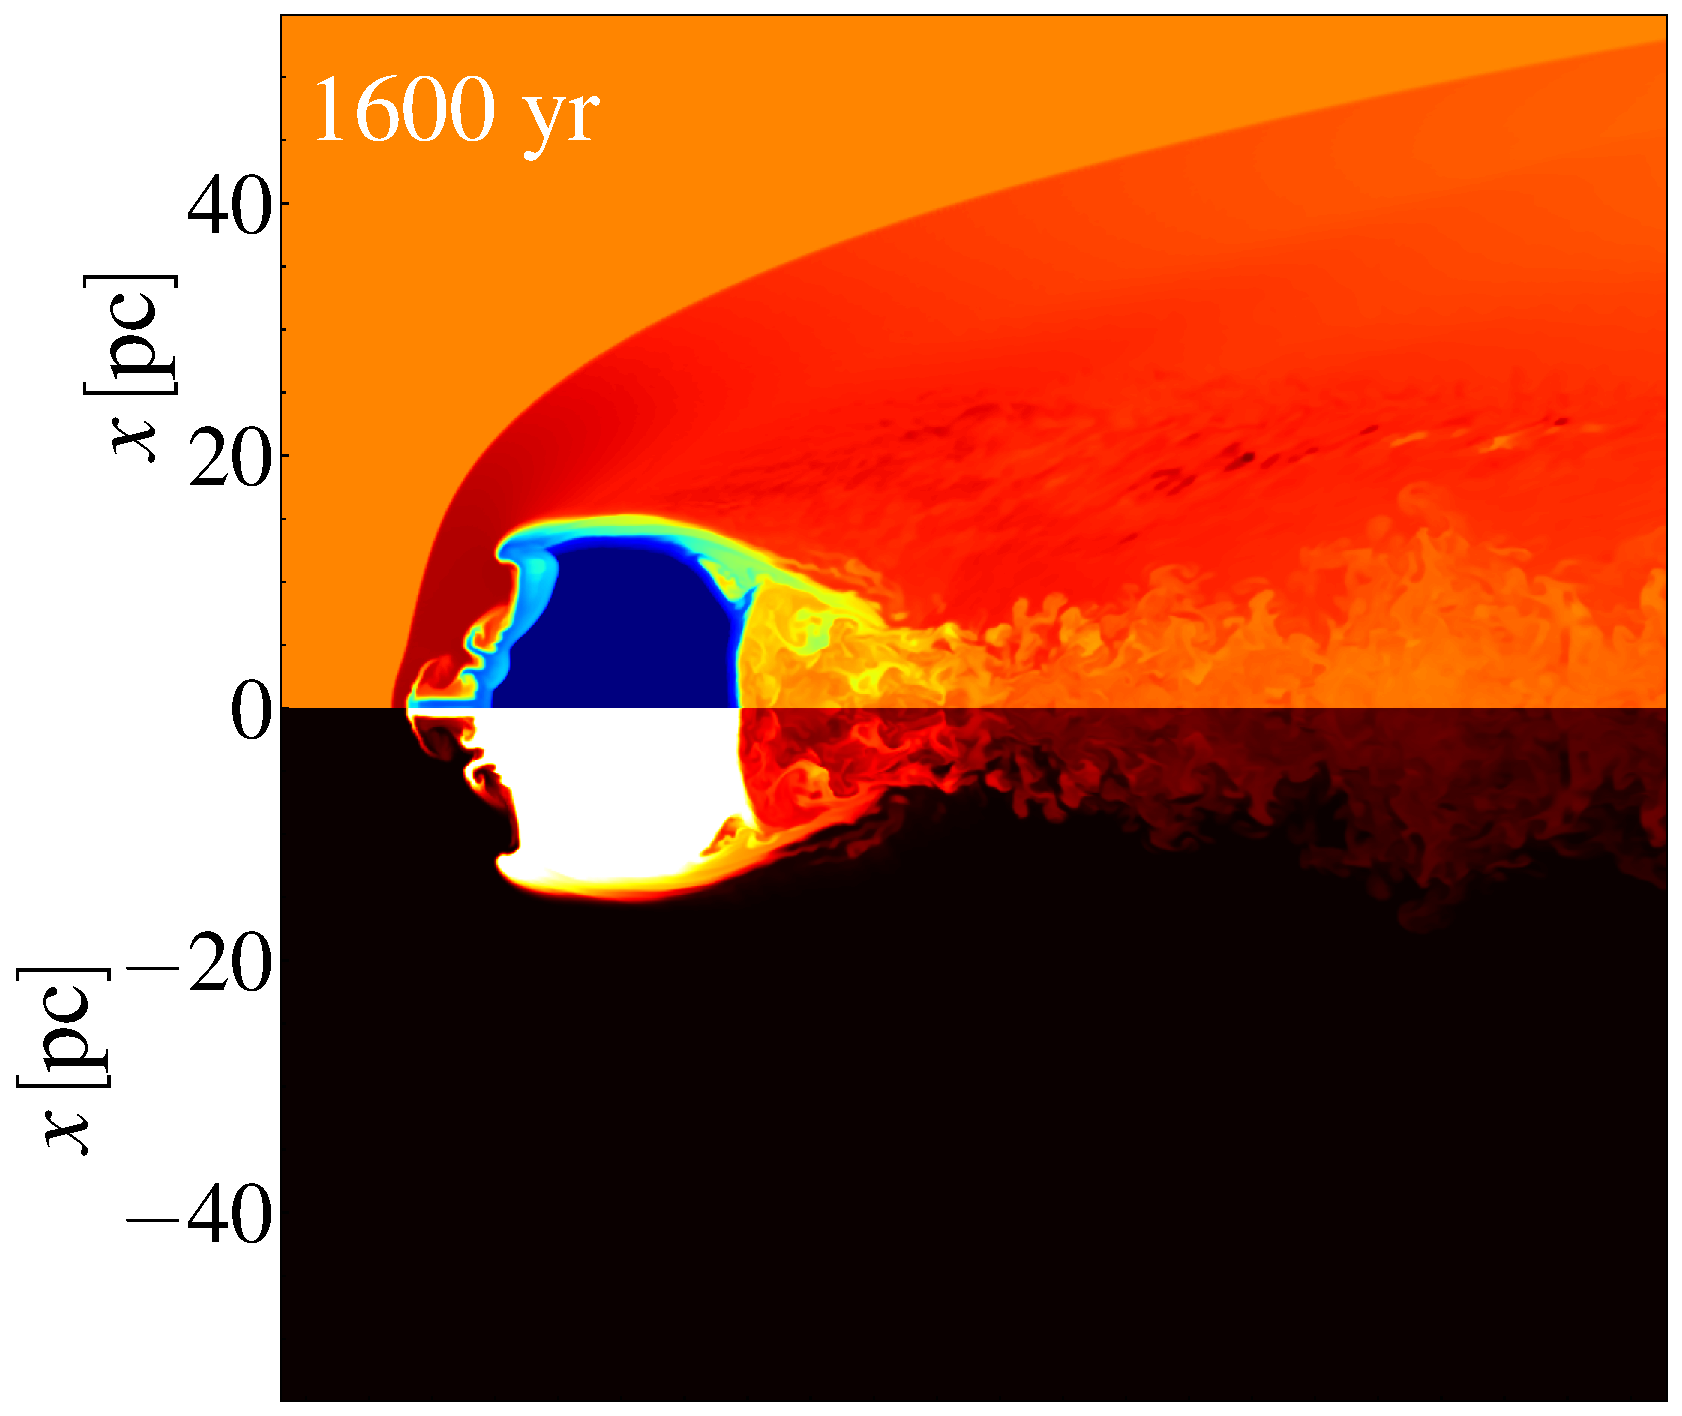
\includegraphics[width=0.3612\linewidth]{images/2d_tem_trac_450.pdf}
	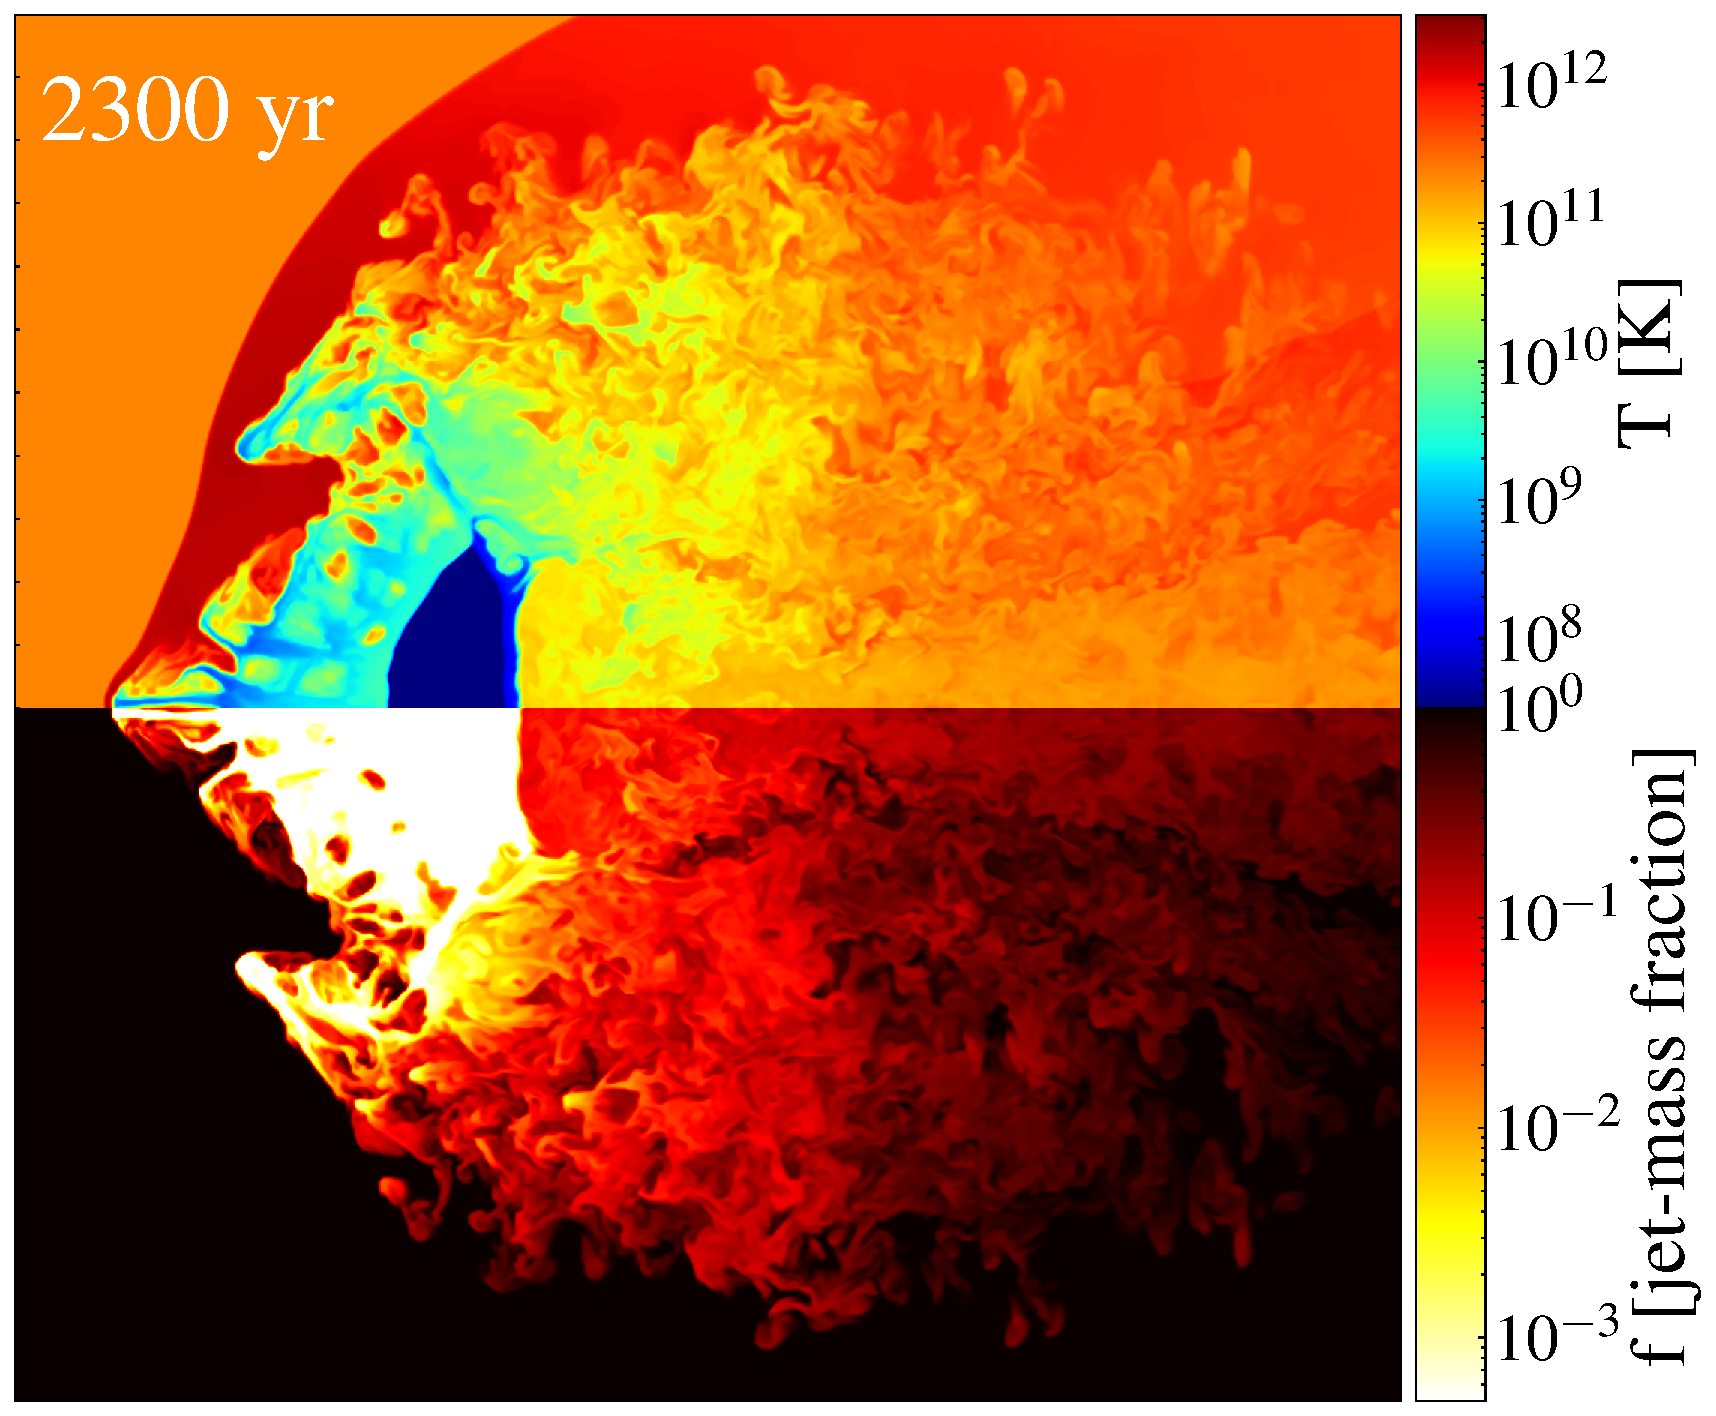
\includegraphics[width=0.3675\linewidth]{images/2d_tem_trac_650.pdf} \\
	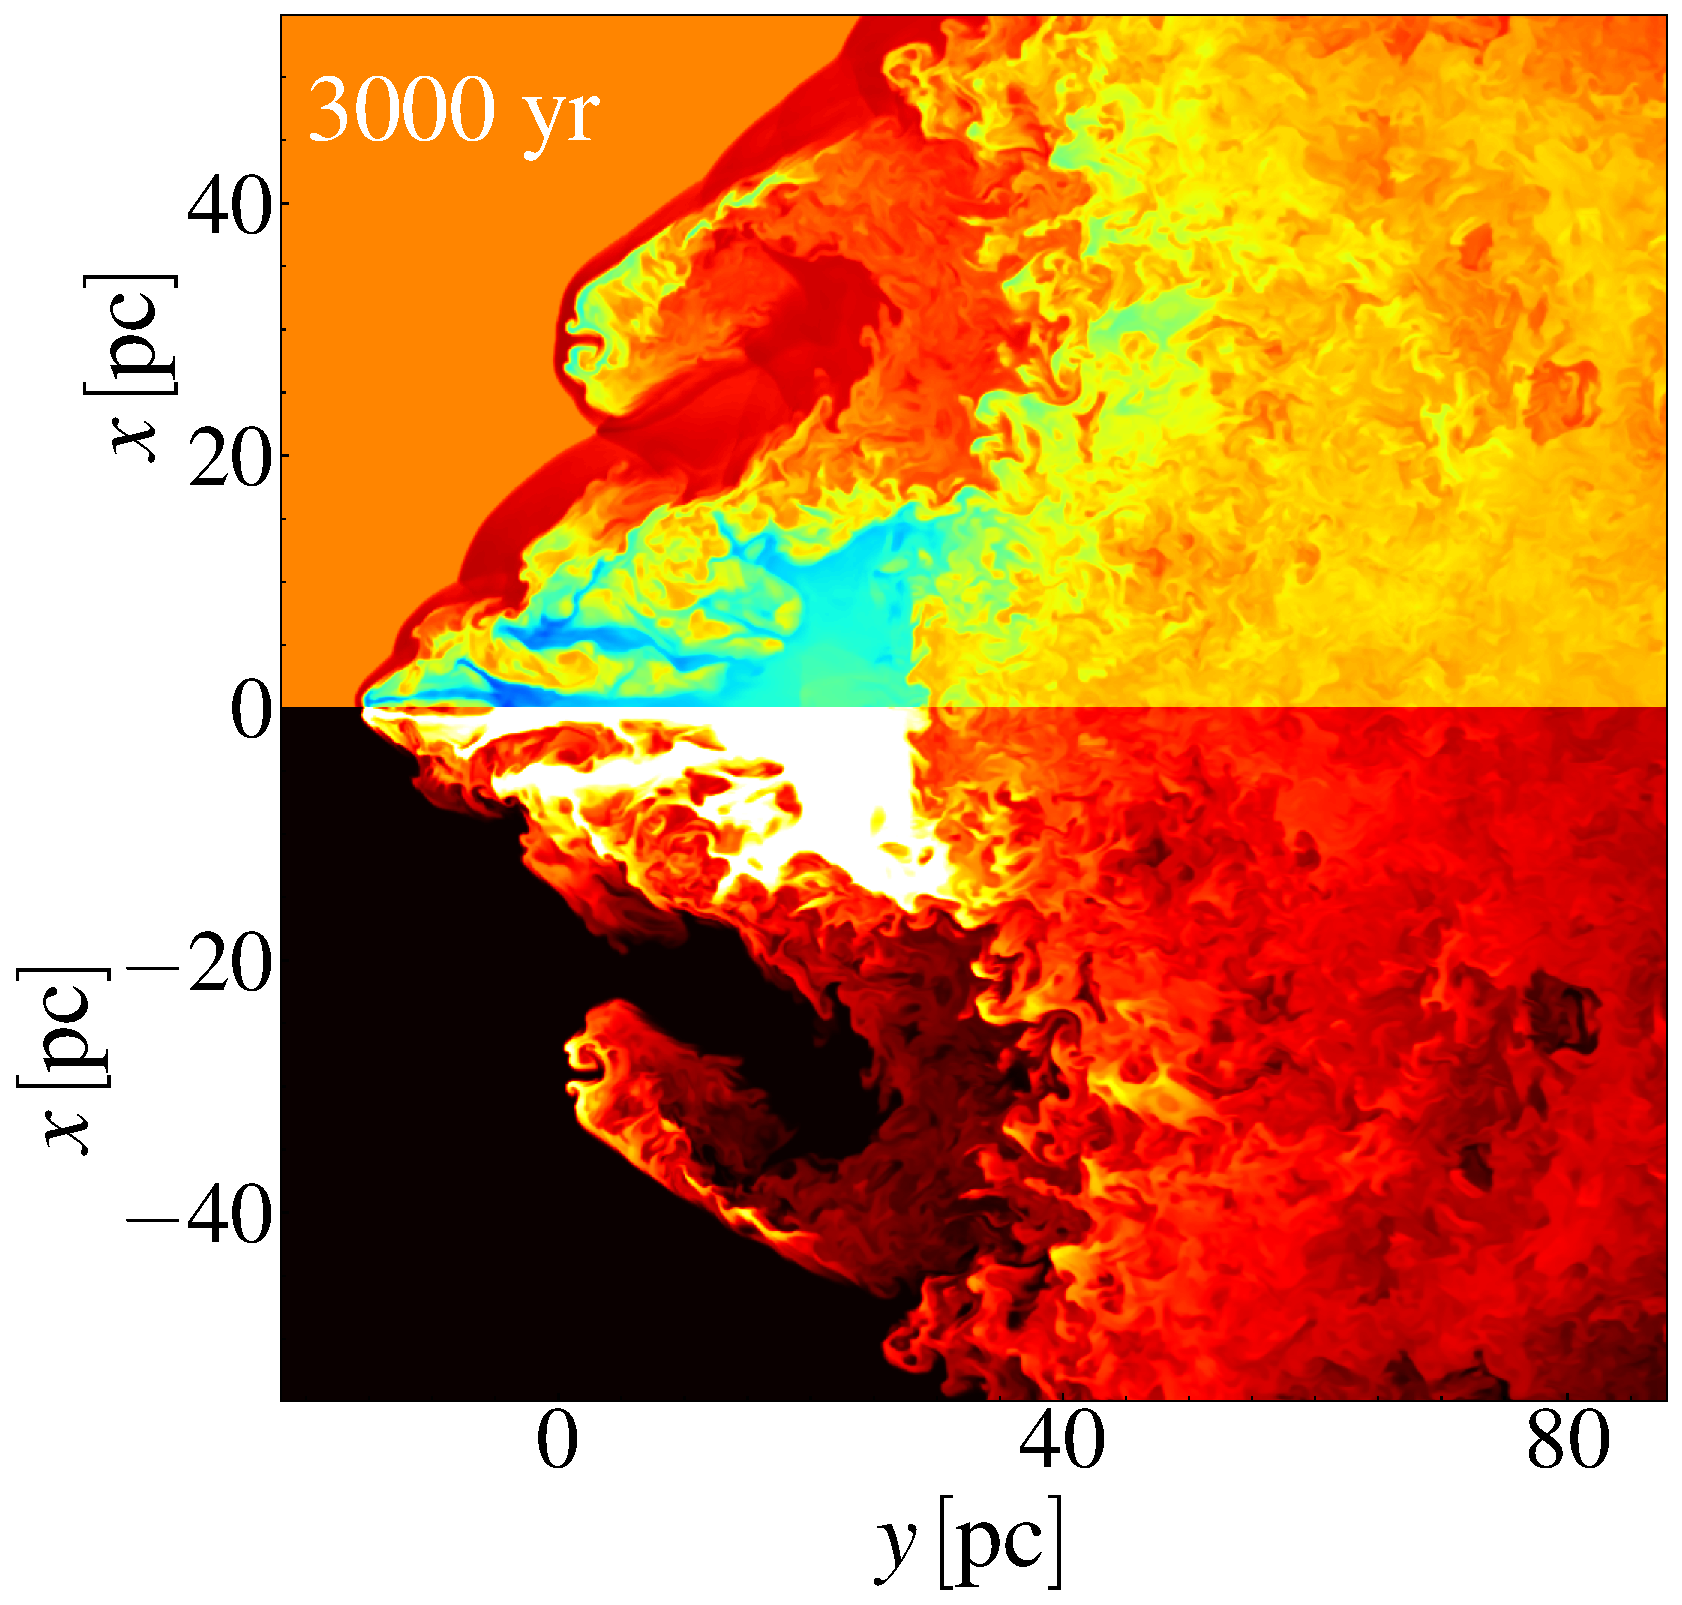
\includegraphics[width=0.36015\linewidth]{images/2d_tem_trac_850.pdf}
	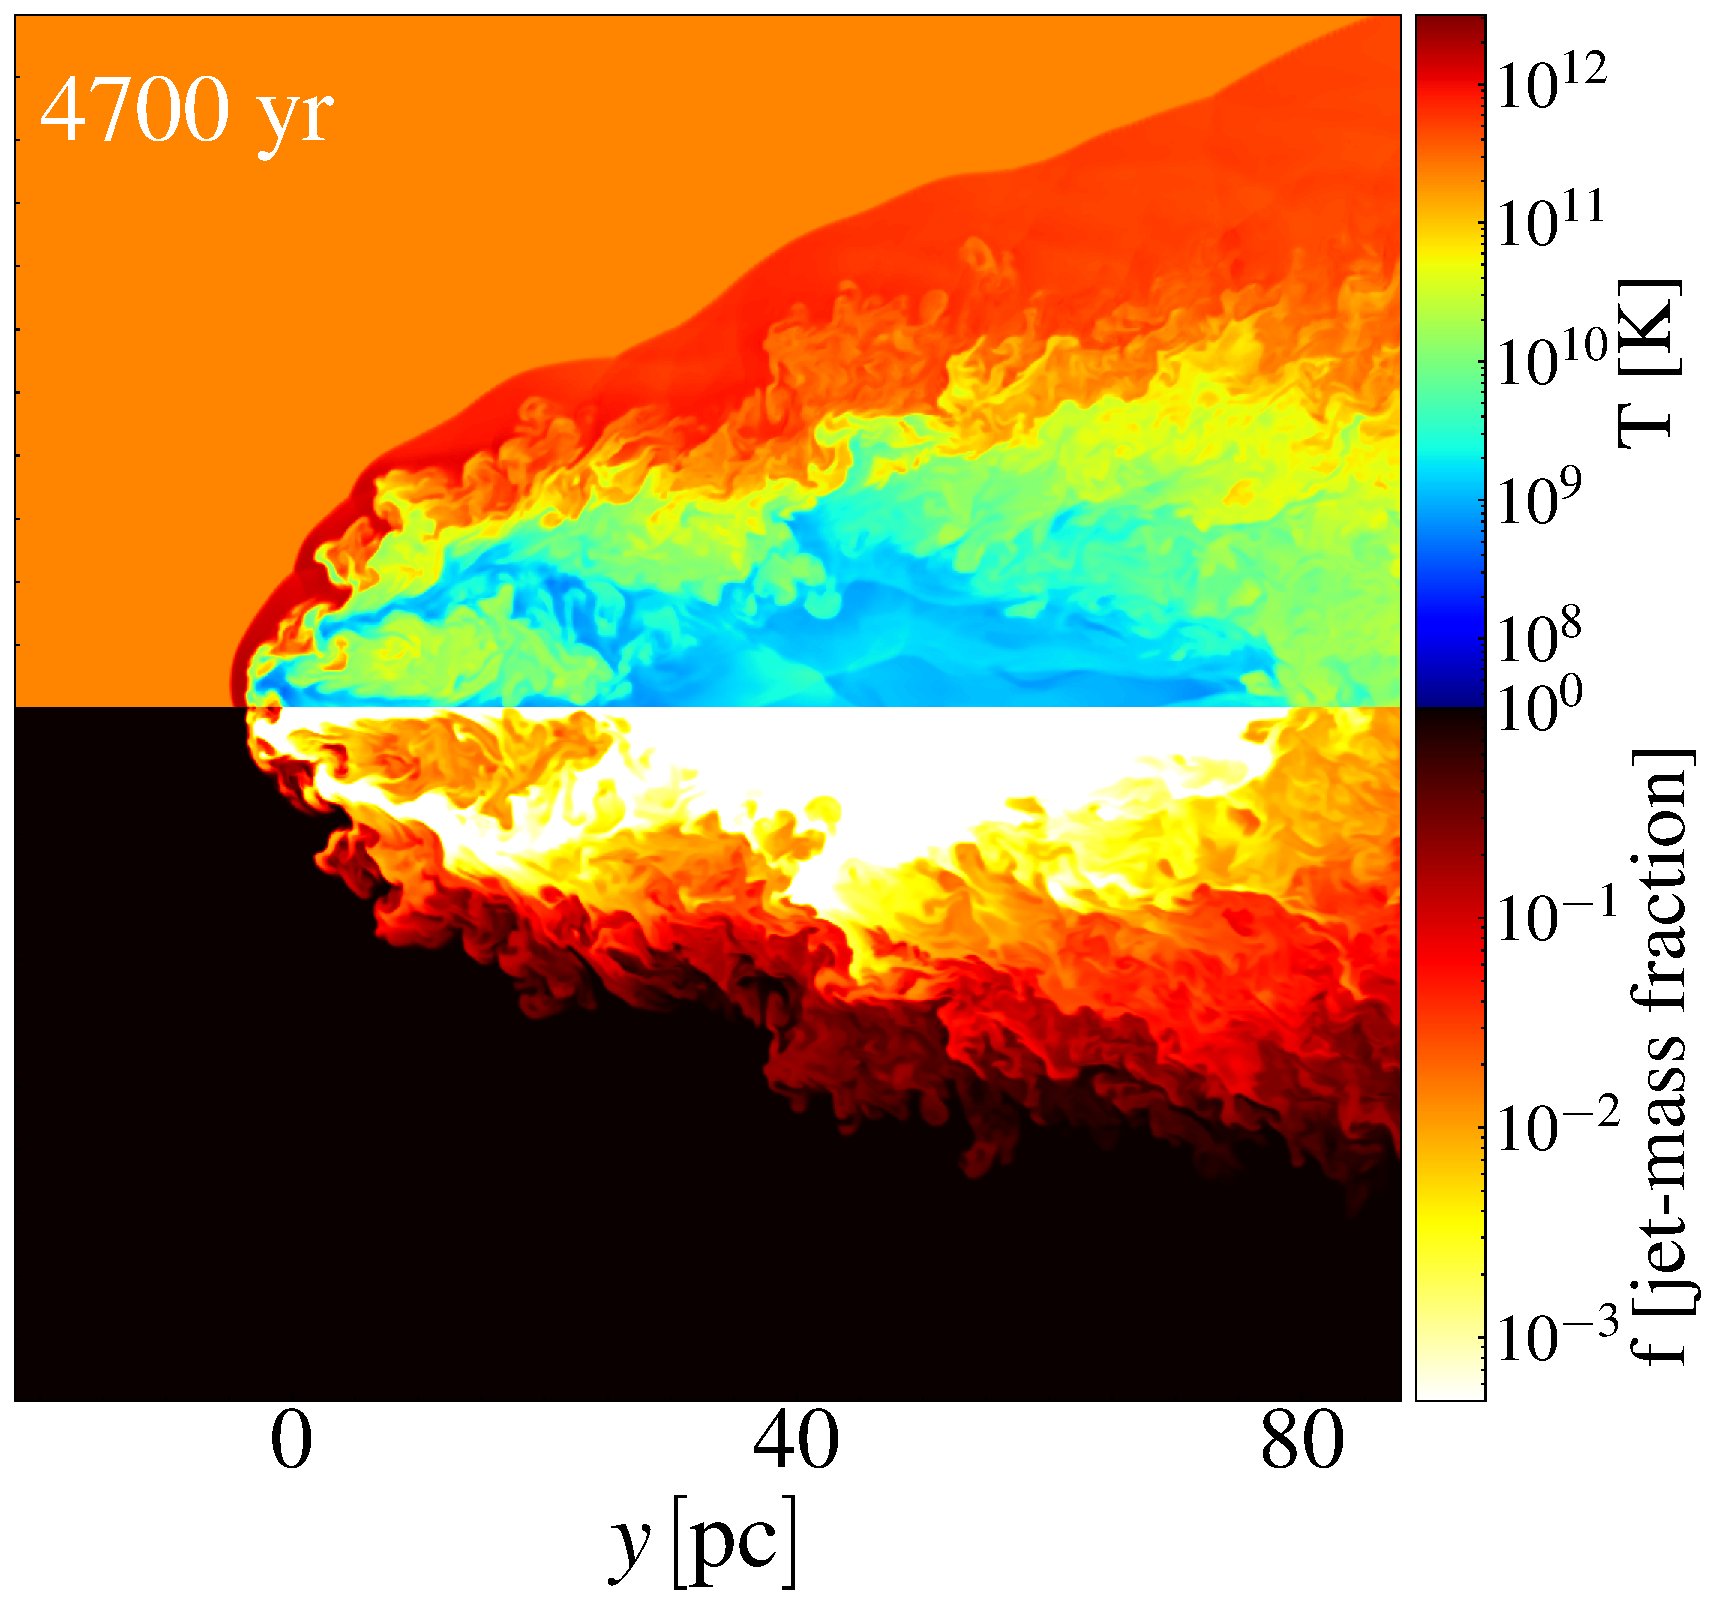
\includegraphics[width=0.36855\linewidth]{images/2d_tem_trac_1300.pdf}
	\end{column}
	\hspace{-3cm}
	\begin{column}{.4\textwidth}
			\begin{block}{Dynamical evolution}
	{\footnotesize
	\begin{itemize}
		\item Free expansion phase
		\item Shock wave and disruption
		\item Important mixing
		\item Ejecta swept away
	\end{itemize}
	}
	\end{block}
	\end{column}
	\end{columns}
\end{frame}

\begin{frame}{Following the time evolution of the interaction}
		
		{\scriptsize Normalized quantities: summing across the outflow boundary and divided by the jet values}
	\begin{columns}
	 \begin{column}{0.5\textwidth}
      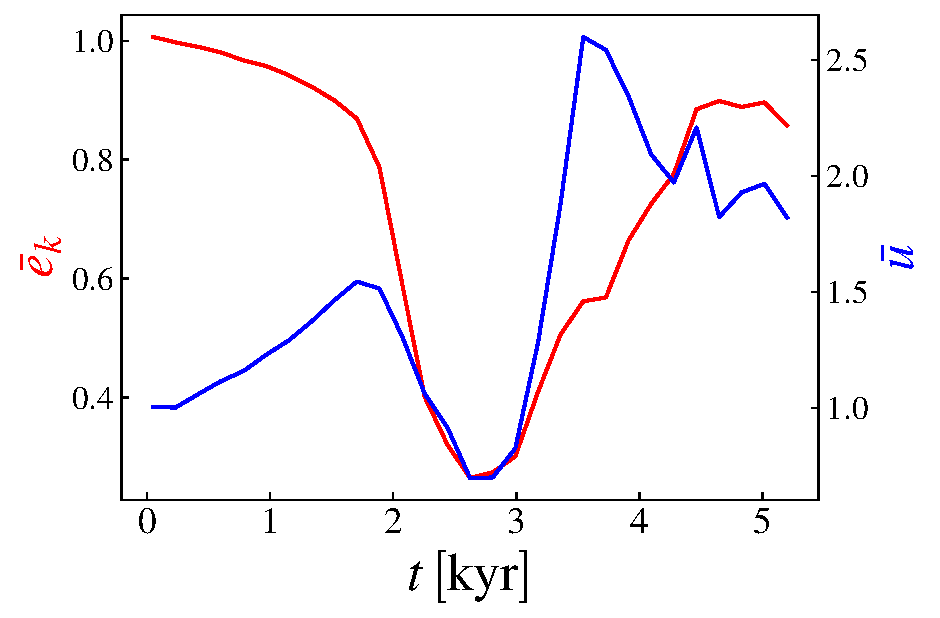
\includegraphics[width=\linewidth]{images/evolution_integrated_xz_u_uk_2_riot.pdf}
     \end{column}
	 \begin{column}{0.5\textwidth}
		{\footnotesize
		\begin{block}{Kinetic and internal energy densities}
			\begin{itemize}
				\item Global drop for both energies
				\item $u \nearrow$ whith the swept heated ejecta 
				\item $e_k \nearrow$ with the heavy matter incorporated
			\end{itemize}
		\end{block}}
	\end{column}
	\end{columns}
	\begin{columns}

	   \begin{column}{.5\textwidth}

      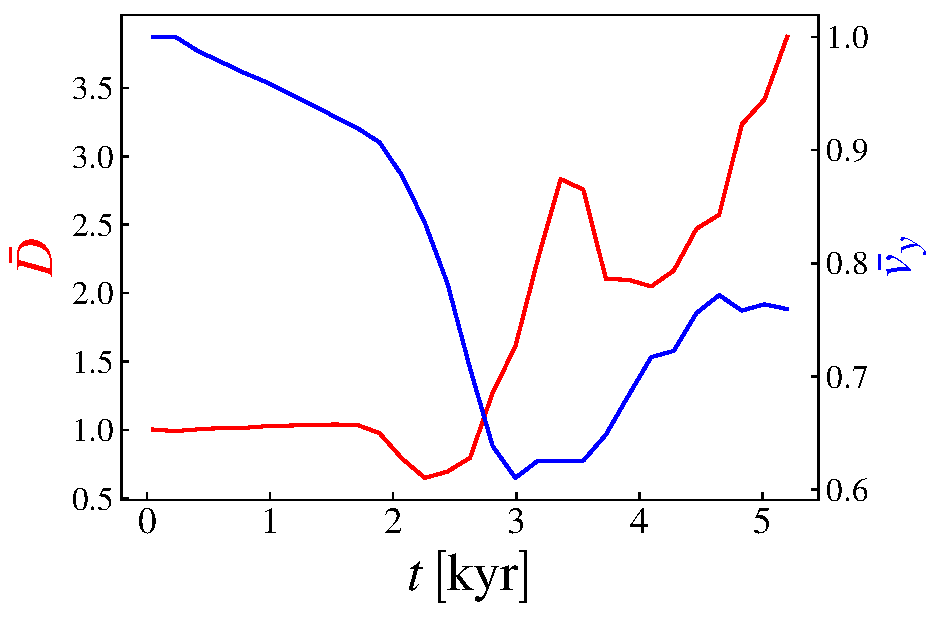
\includegraphics[width=\linewidth]{images/evolution_integrated_xz_d_vy_2_riot.pdf}
	   \end{column}
	   \begin{column}{.5\textwidth}
		{\footnotesize
		\begin{block}{Lab frame density and axial velocity}
			\begin{itemize}
				\item $D \nearrow$ with the entrainment of the ejecta
				\item $v_y \searrow$ with the disruption then $\nearrow$ with the reacceleration
			\end{itemize}
		\end{block}}
	   \end{column}
	\end{columns}
\end{frame}

\section{Non-thermal emissions}

\begin{frame}{Non-thermal emission:\\
	Simplified approach to compute the radiative output}
	\begin{columns}
		{\scriptsize
		\begin{column}{.5\textwidth}
			\begin{block}{Power emitted}
				\begin{itemize}
					\item Non-thermal energy $E_{\rm NT} = \eta U_{\rm cell}$ where $\eta<1$
					\item Broken power-law for the e$^{-}$ distribution with a break 
							energy given by the adiabatic time  \\
					\item Inverse Compton scattering + Synchrotron
				\end{itemize}
			\end{block}
			\begin{block}{Inverse Compton scattering}
			    \begin{itemize}
				    \item Target photons:\\
						$\rightarrow$ Anisotropic CMB + IR galactic background
					\item Approximate formula for the Thompson+Klein-Nishina regime
						(Khangulyan 2014, Bosch-Ramon 2018)
				\end{itemize}
			\end{block}
		\end{column}
		\begin{column}{.5\textwidth}
			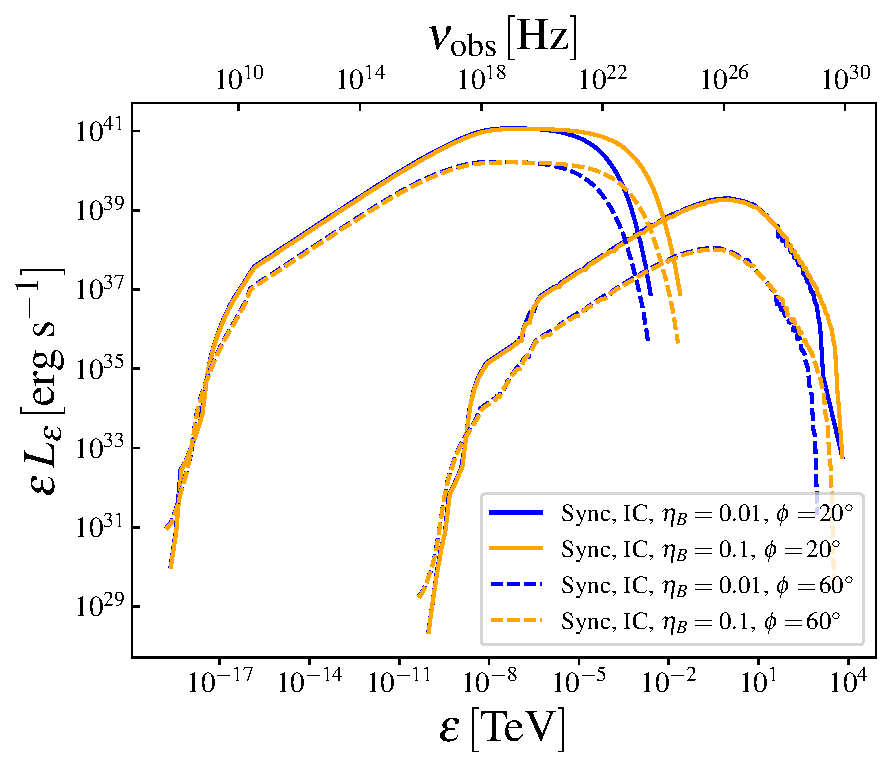
\includegraphics[width=\linewidth]{images/eled_hr.pdf}
			\begin{exampleblock}{Emitted luminosity}
				\begin{itemize}
					\item With the given e$^{-}$ distribution, we reach the PeV in IC
					\item The Synchrotron emission reaches $10^{41}\,{\rm erg}\,{\rm s}^{-1}$
							and the IC $10^{39}\,{\rm erg}\,{\rm s}^{-1}$
				\end{itemize}
			\end{exampleblock}
			\centering
		\end{column}
		}
	\end{columns}
\end{frame}
\begin{frame}{Flux on the line of sight for a source at $z=0.007$ and $\phi=20$°}
	\begin{columns}
		\begin{column}{0.1\textwidth}
				{\small {\bf IC} \\$10^{27}\,{\rm Hz}$  }
		\end{column}
		\begin{column}{\textwidth}
	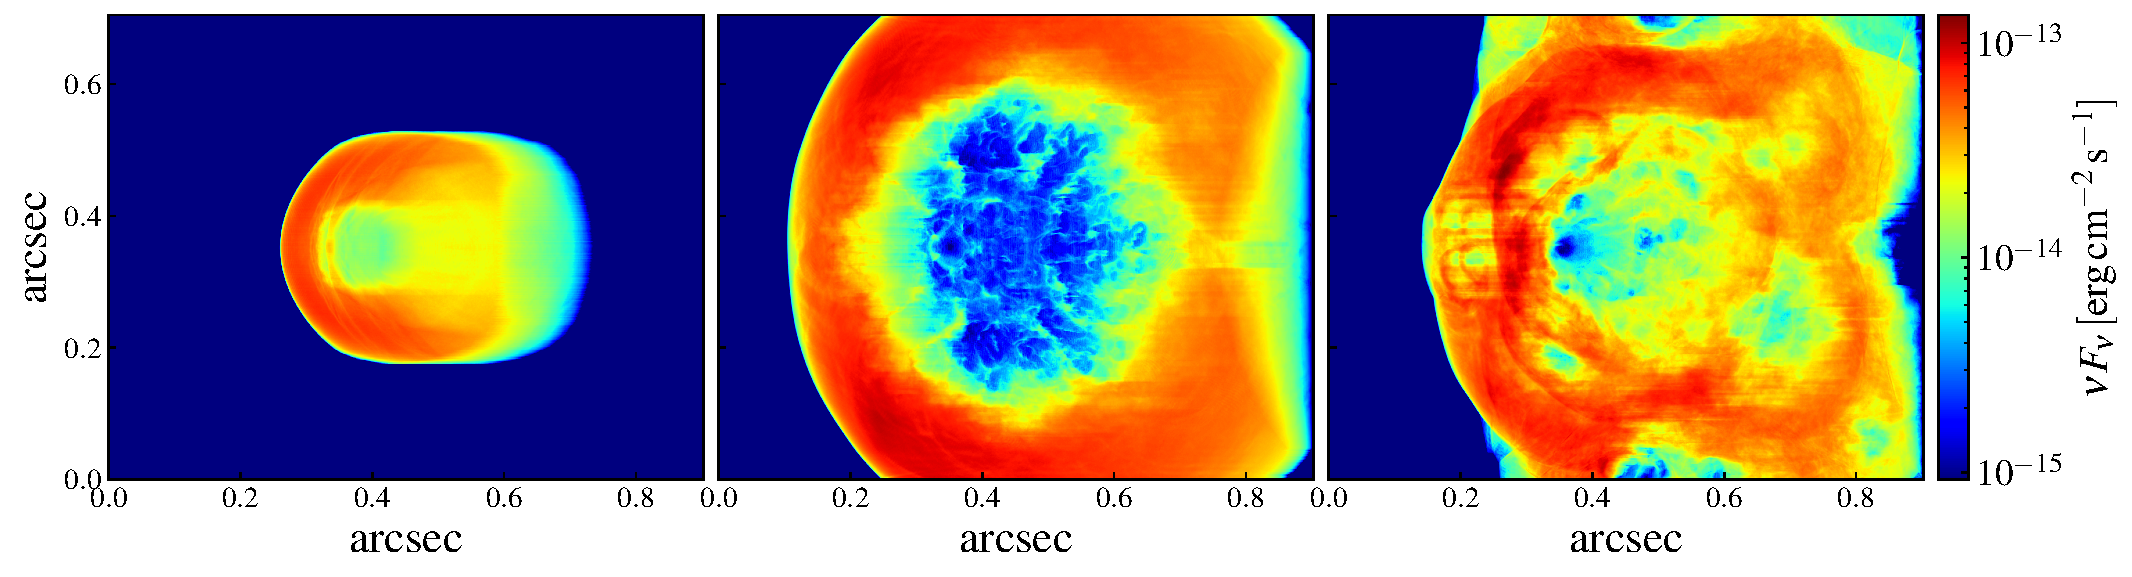
\includegraphics[width=\linewidth]{images/2dmaps/2Dmap_flux_freq_27_dist_31_phi_20_ic.pdf}
		\end{column}
	\end{columns}
	\begin{columns}
		\begin{column}{0.1\textwidth}
				{\small{\bf Sync} \\ $10^{10}\,{\rm Hz}$}
		\end{column}
		\begin{column}{\textwidth}

	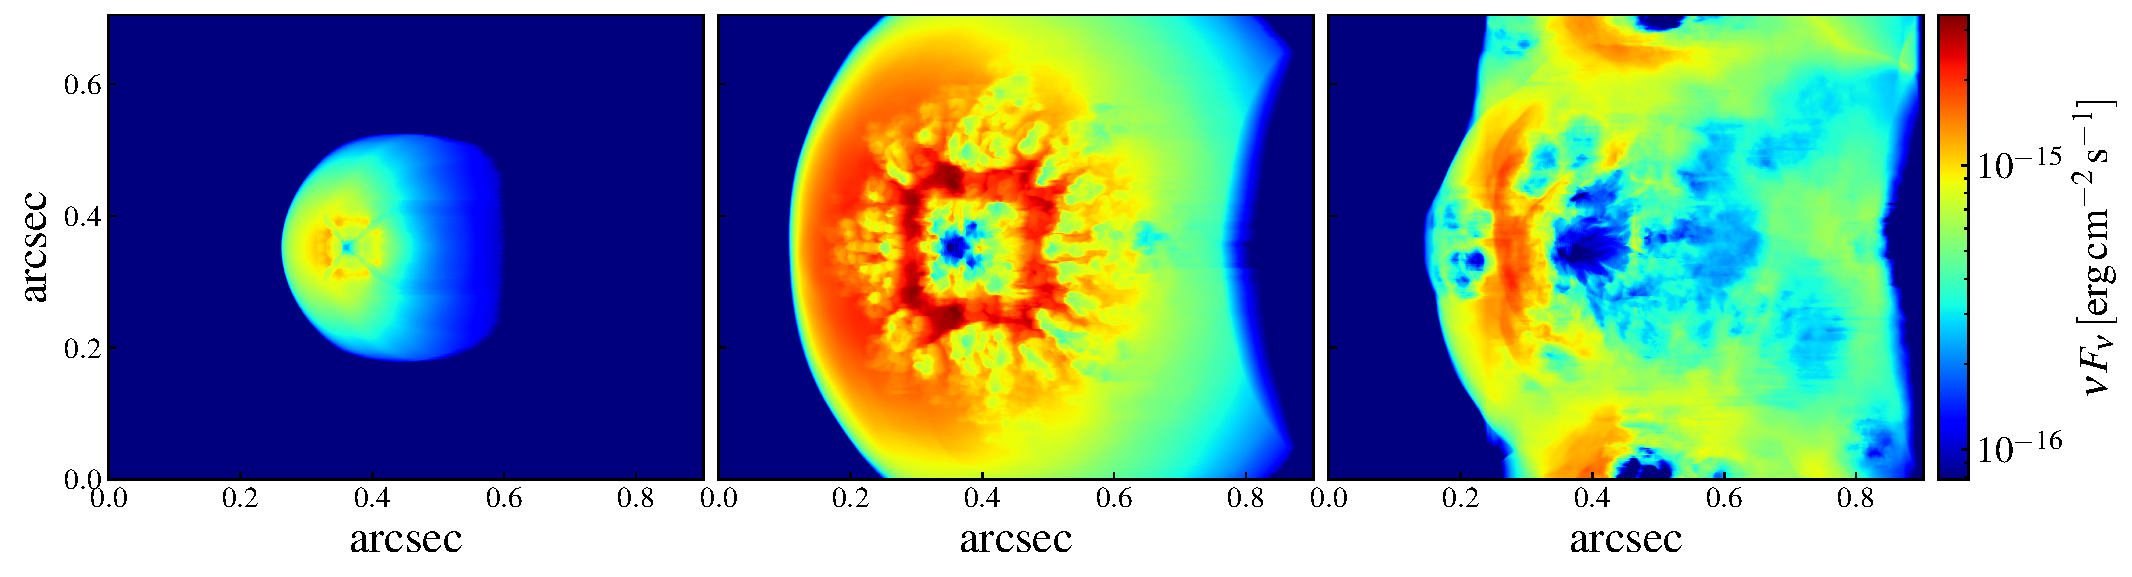
\includegraphics[width=\linewidth]{images/2dmaps/2Dmap_flux_freq_10_dist_31_phi_20_sync.pdf}
		\end{column}
	\end{columns}
	\vspace{8pt}
		\hspace{70pt} $1\,{\rm kyr}$ \hspace{60pt} $2\,{\rm kyr}$ \hspace{60pt} $2.9\,{\rm kyr}$
\end{frame}

\begin{frame}{Flux on the line of sight for a source at $z=0.007$ and $\phi=60$°}
	\begin{columns}
		\begin{column}{0.1\textwidth}
				{\small {\bf IC} \\$10^{24}\,{\rm Hz}$  }
		\end{column}
		\begin{column}{\textwidth}
	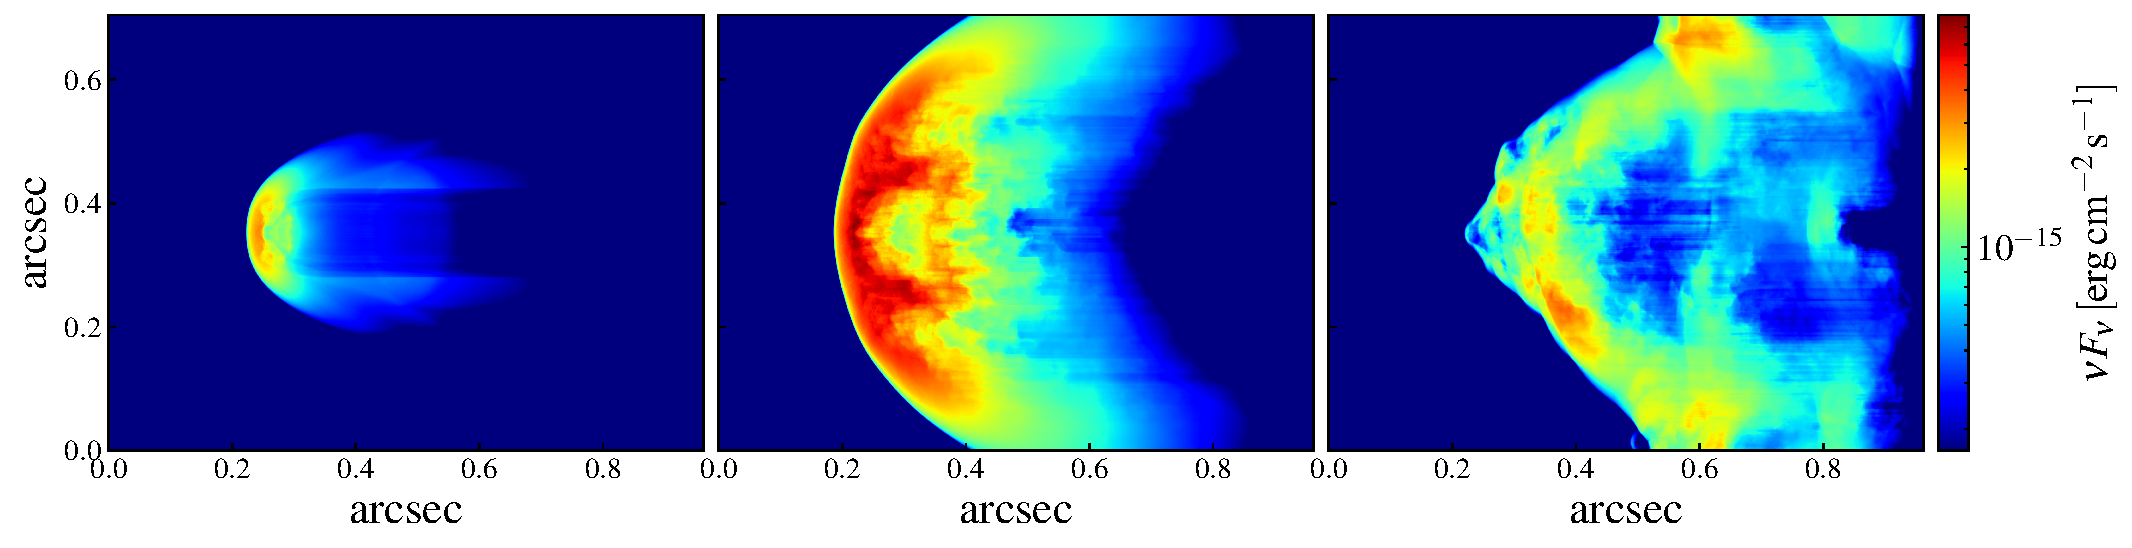
\includegraphics[width=\linewidth]{images/2dmaps/2Dmap_flux_freq_24_dist_31_phi_60_ic.pdf}
		\end{column}
	\end{columns}
	\begin{columns}
		\begin{column}{0.1\textwidth}
				{\small{\bf Sync} \\ $10^{18}\,{\rm Hz}$}
		\end{column}
		\begin{column}{\textwidth}

	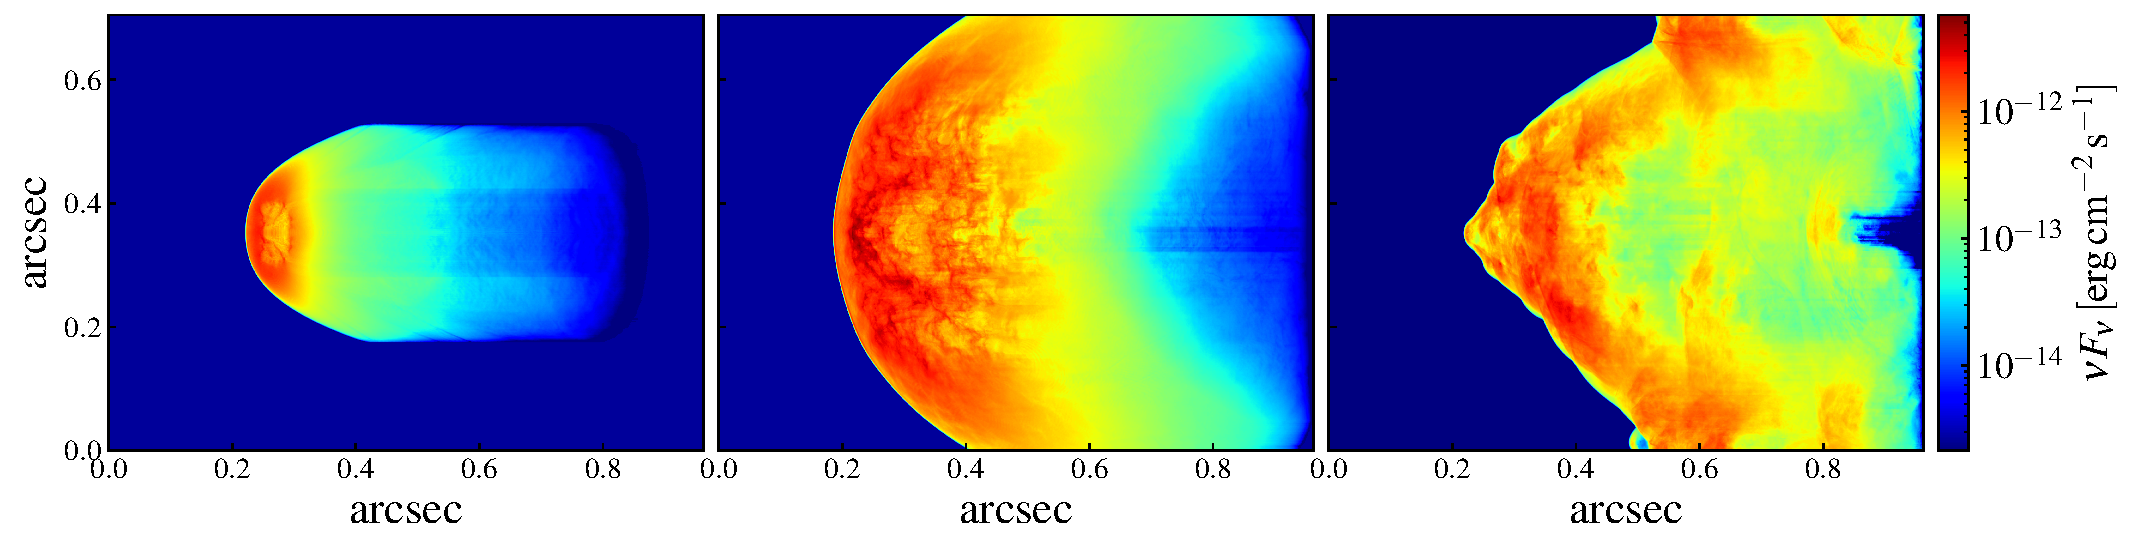
\includegraphics[width=\linewidth]{images/2dmaps/2Dmap_flux_freq_18_dist_31_phi_60_sync.pdf}
		\end{column}
	\end{columns}
	\vspace{8pt}
		\hspace{70pt} $1\,{\rm kyr}$ \hspace{60pt} $2\,{\rm kyr}$ \hspace{60pt} $2.9\,{\rm kyr}$
\end{frame}

\begin{frame}{SEDs with $\phi=20,60^{\circ}$}
	\begin{columns}
		\begin{column}{.6\textwidth}
			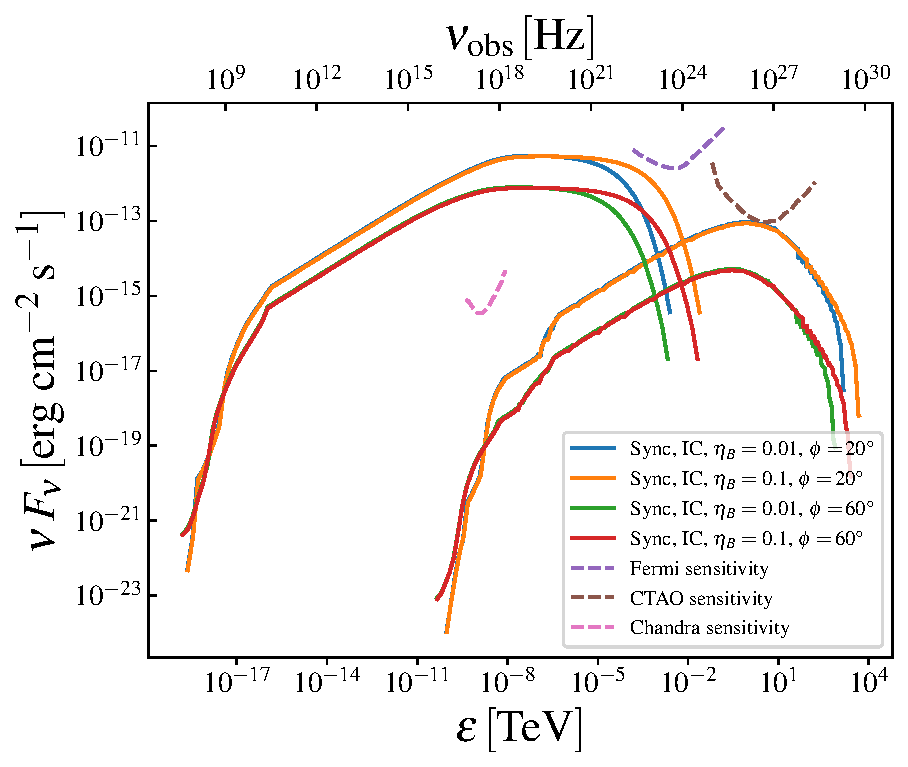
\includegraphics[width=\textwidth]{images/sed_hr.pdf}
		\end{column}
		\begin{column}{.4\textwidth}
			{\scriptsize
			\begin{itemize}
				\item Ratio $\eta_{\rm B}=p_{\rm B}/p_{\rm g}=10^{-2}$
				\item Source at $z=0.003\;(13{\rm Mpc})$ (type CenA)
				\item Fluxes for Synchrotron and IC emission
				\item Possible detecion of Sync by Chandra and IC by CTAO
			\end{itemize}
			}
		\end{column}
	\end{columns}
\end{frame}

\begin{frame}{Light curve with $\phi=20,60^{\circ}$ and $z=0.007\;(31{\rm Mpc})$}
	\begin{columns}
		\begin{column}{.5\textwidth}
		\centering
		{\scriptsize Xrays $(10^{18}\,{\rm GHz})$}
			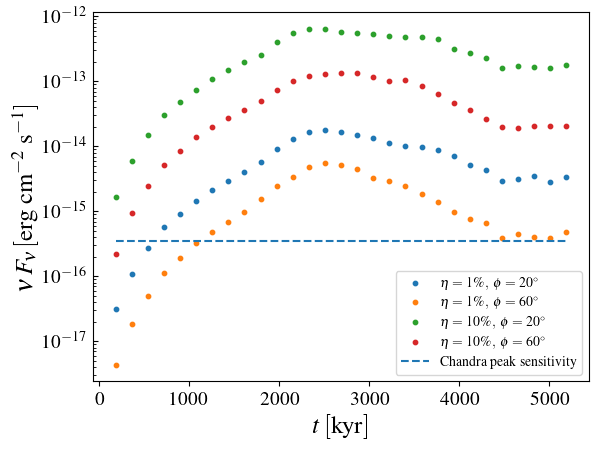
\includegraphics[width=.95\textwidth]{images/Chandra_Sync.png}
		\end{column}
		\begin{column}{.5\textwidth}
				\centering
          {\scriptsize $\gamma$-rays $(10^{27}\,{\rm GHz})$}
   	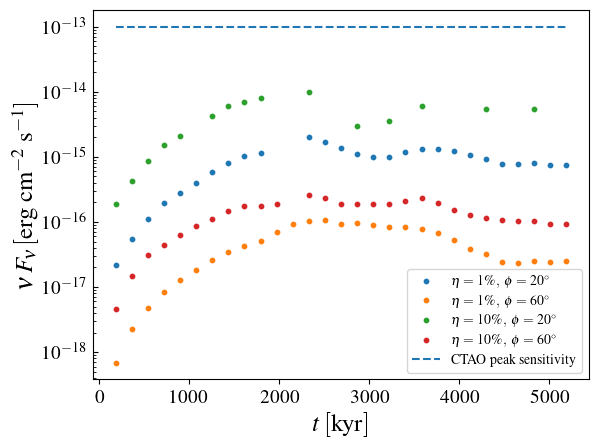
\includegraphics[width=.95\textwidth]{images/CTAO_IC.png}
		\end{column}
	\end{columns}
		{\scriptsize
			\begin{itemize}
				\item Internal to non-thermal energy ratio $\eta=0.1,0.01$ 
				
			\end{itemize}
		}
\end{frame}


\section{To take away}
\begin{frame}
	\begin{columns}
		{\scriptsize
		\begin{column}{0.5\textwidth}
			\begin{block}{Simulations}
					\textbf{Jet/SN interaction}
				\begin{itemize}
					\item A post-disruption expansion of the bow-shock, who covers the whole jet
					\item Provokes a jet speed local deceleration of $40\%$
					\item Results in a mass-load of $10^{-4}\,M_{\odot}\,{\rm yr}^{-1}$
					      over the interaction time scale 
					\item Strong mixing with the jet flow after the disruption
				\end{itemize}

		\textbf{Ongoing work} 
			\begin{itemize}
				\item SN exploding close to the jet walls, triggering mixing with the ISM
				\item Add $\vec{B}$ to the simulations with \texttt{Lostrego} (L\'opez-Miralles 2022)
			\end{itemize}
			\end{block}


		\end{column}
			\hspace{-.5cm}
		\begin{column}{0.6\textwidth}
			\begin{exampleblock}{Radiative outcomes}
				\begin{itemize}
					\item Computation of the high energy 
							non-thermal emissions using simplified models\\ (Khangulyan 2014, Bosch-Ramon 2018)
					\item Estimate the possibilities of detection of the 
							current and future detectors (CTAO, Chandra, VLA, etc..) for nearby sources
				\end{itemize}
			\end{exampleblock}

			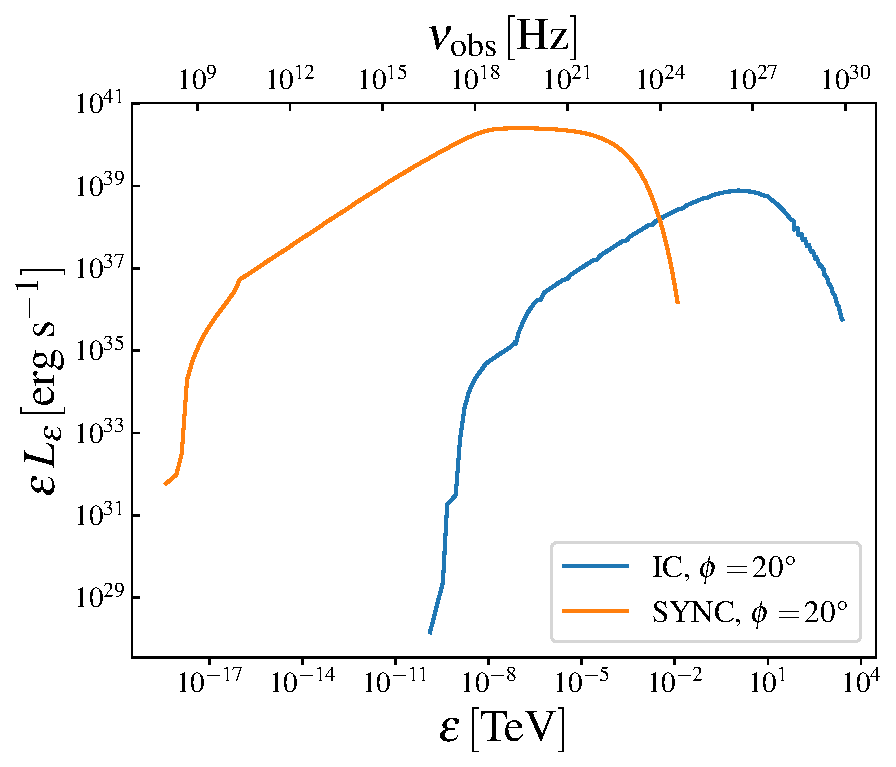
\includegraphics[width=.8\linewidth]{images/eled_ic_sync_hr.pdf}
			\centering
				{\scriptsize Preliminary work on the simulations results}

		\end{column}}
	\end{columns}
\end{frame}

%\section{Backup}

\begin{frame}{Non-thermal emission:\\
	Simplified approach to compute the radiative output}
	\begin{columns}
		{\scriptsize
		\begin{column}{.5\textwidth}
			\begin{block}{Power emitted}
				\begin{itemize}
					\item Non-thermal energy $E_{\rm NT} = \eta U_{\rm cell}$ where $\eta<1$
					\item Broken power-law for the e$^{-}$ distribution with a break 
							energy given by the adiabatic time  \\
					\item \textcolor{blue}{Inverse Compton scattering} + \textcolor{red}{Synchrotron}
%					\quad\quad\quad $N\propto\left\{
%							\begin{array}{ll}
%								E^{-p} & E<E_b\\
%								E^{-(p+1)} & E>E_b
%							\end{array}
%							\right.$

				\end{itemize}
			\end{block}
			\begin{block}{Inverse Compton scattering}
			    \begin{itemize}
				    \item Target photons:\\
						$\rightarrow$ Anisotropic CMB + IR galactic background
					\item Approximate formula for the Thompson+Klein-Nishina regime
						(Khangulyan 2014, Bosch-Ramon 2018)
				\end{itemize}
			\end{block}
		\end{column}
		\begin{column}{.5\textwidth}
			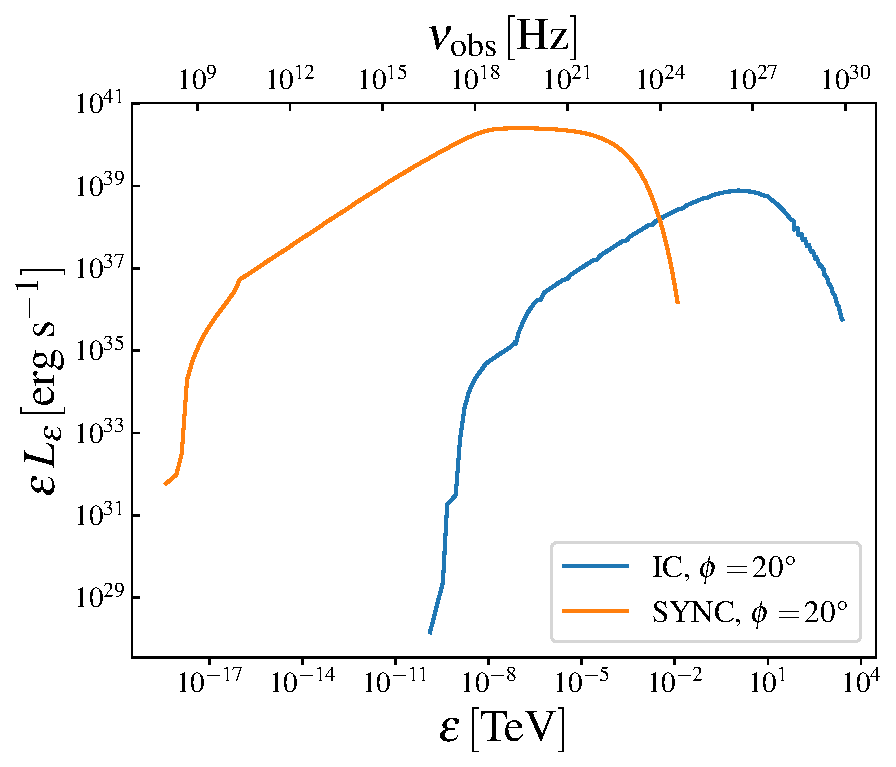
\includegraphics[width=\linewidth]{images/eled_ic_sync_hr.pdf}
			\begin{exampleblock}{SEDs}
				\begin{itemize}
					\item With the given e$^{-}$ distribution, we reach the PeV in IC
					\item The \textcolor{red}{Synchrotron} emission reaches $10^{40}\,{\rm erg}\,{\rm s}^{-1}$
							and the \textcolor{blue}{IC}  $10^{38}\,{\rm erg}\,{\rm s}^{-1}$
				\end{itemize}
			\end{exampleblock}
			\centering
		\end{column}
		}
	\end{columns}
\end{frame}
\begin{frame}{Flux on the line of sight for a source at $z=0.01$ and $\phi=20$°}
	\begin{columns}
		\begin{column}{0.1\textwidth}
				{\small {\bf IC} \\$10^{26}\,{\rm Hz}$  }
		\end{column}
		\begin{column}{\textwidth}
	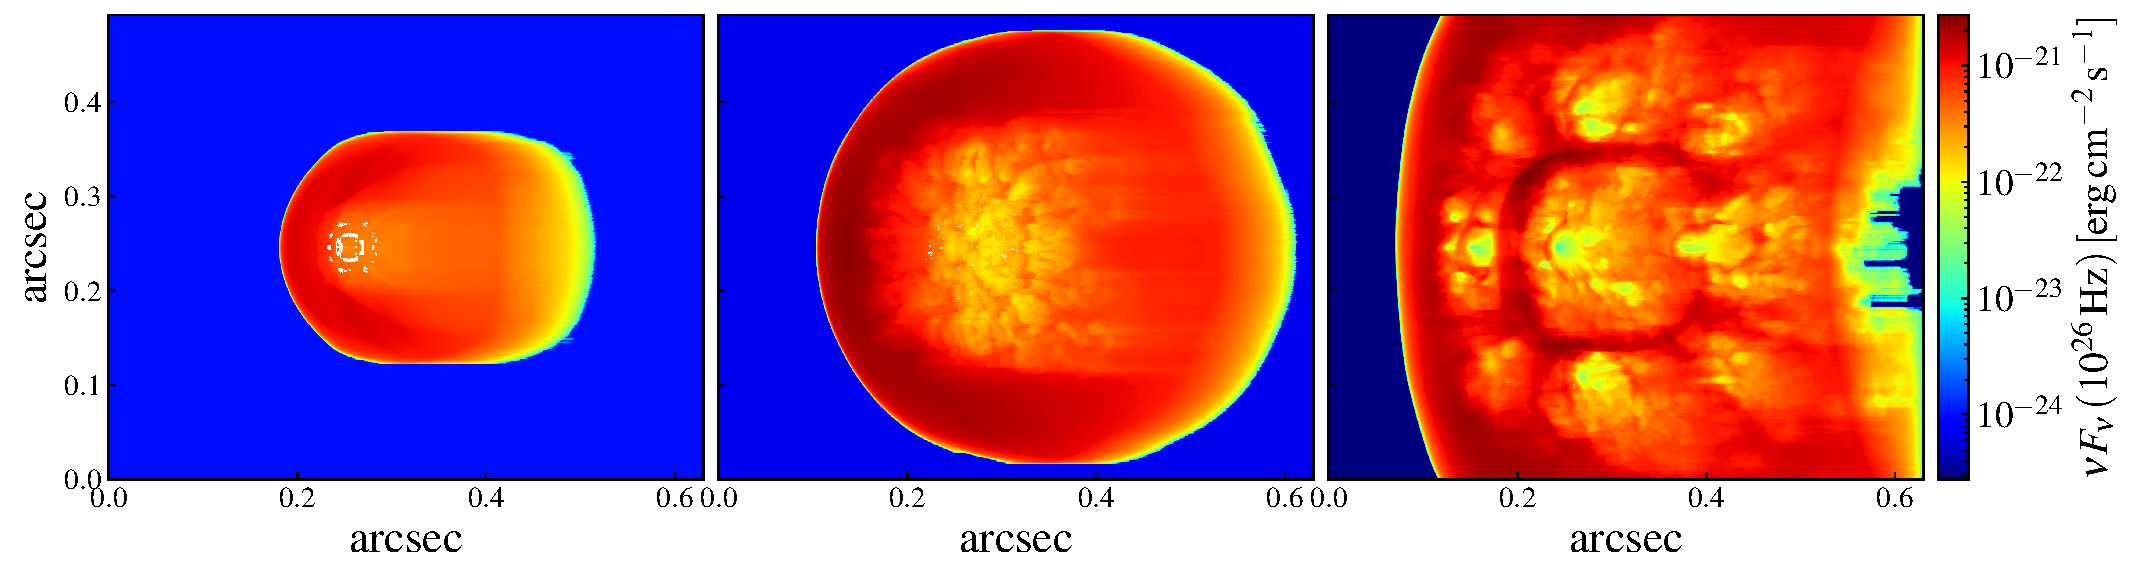
\includegraphics[width=\linewidth]{images/inte_flux_26_ic_5_10_15.pdf}
		\end{column}
	\end{columns}
	\begin{columns}
		\begin{column}{0.1\textwidth}
				{\small{\bf Sync} \\ $10^{20}\,{\rm Hz}$}
		\end{column}
		\begin{column}{\textwidth}
            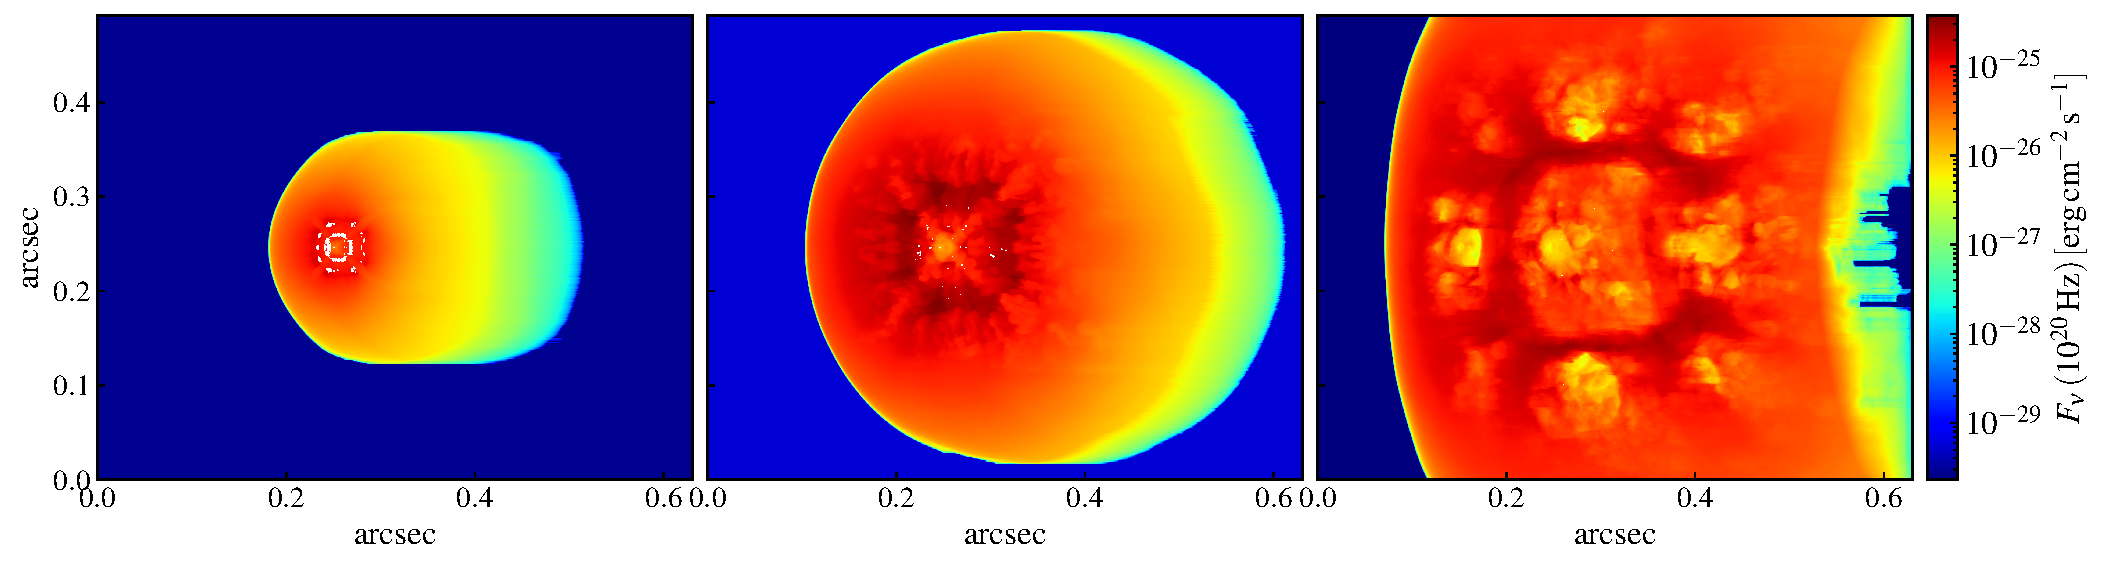
\includegraphics[width=\linewidth]{images/inte_flux_20_sync_5_10_15.pdf}
		\end{column}
	\end{columns}
	\vspace{8pt}
		\hspace{70pt} $1\,{\rm kyr}$ \hspace{60pt} $2\,{\rm kyr}$ \hspace{60pt} $2.9\,{\rm kyr}$
\end{frame}



\begin{frame}{Following the time evolution of the interaction}
		
		{\scriptsize Normalized quantities: summing across the outflow boundary and divided by the jet values}
	\begin{columns}
	 \begin{column}{0.5\textwidth}
      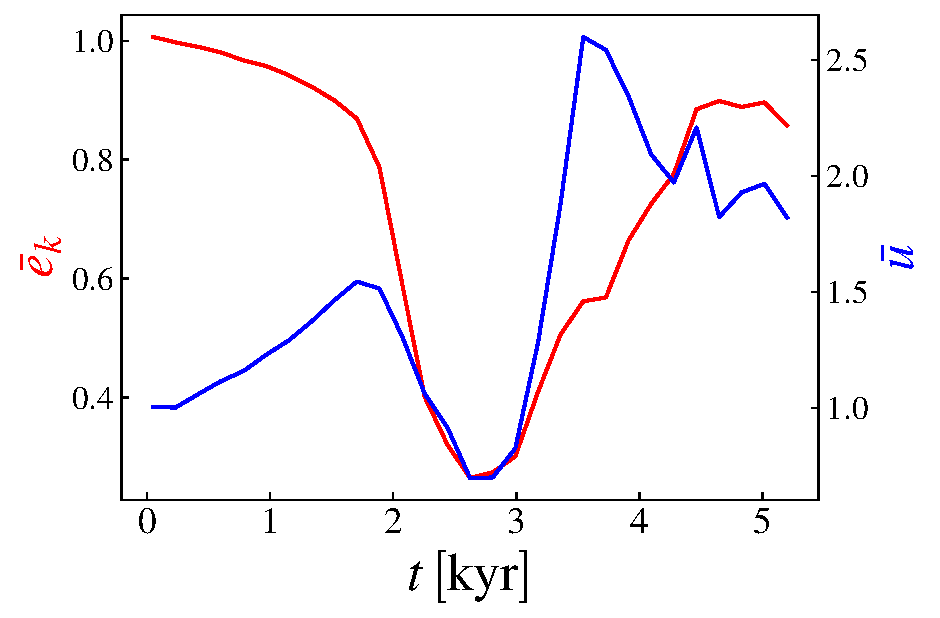
\includegraphics[width=\linewidth]{images/evolution_integrated_xz_u_uk_2_riot.pdf}
     \end{column}
	 \begin{column}{0.5\textwidth}
		{\footnotesize
		\begin{block}{Kinetic and internal energy densities}
			\begin{itemize}
				\item Global drop for both energies
				\item $u \nearrow$ whith the swept heated ejecta 
				\item $e_k \nearrow$ with the heavy matter incorporated
			\end{itemize}
		\end{block}}
	\end{column}
	\end{columns}
	\begin{columns}

	   \begin{column}{.5\textwidth}

      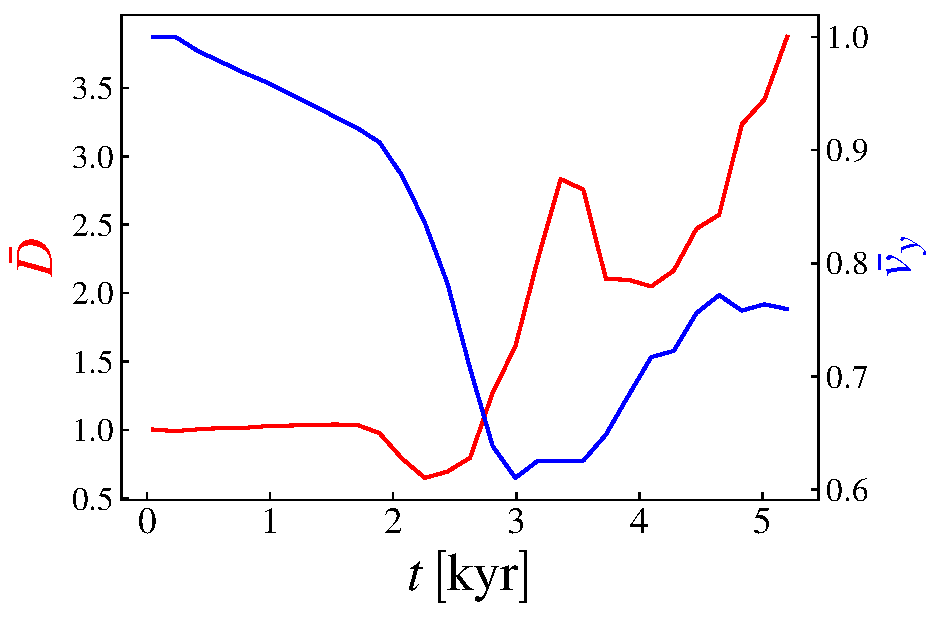
\includegraphics[width=\linewidth]{images/evolution_integrated_xz_d_vy_2_riot.pdf}
	   \end{column}
	   \begin{column}{.5\textwidth}
		{\footnotesize
		\begin{block}{Lab frame density and axial velocity}
			\begin{itemize}
				\item $D \nearrow$ with the entrainment of the ejecta
				\item $v_y \searrow$ with the disruption then $\nearrow$ with the reacceleration
			\end{itemize}
		\end{block}}
	   \end{column}
	\end{columns}
\end{frame}

\begin{frame}{RHD equations}
\begin{columns}
\begin{column}{0.5\textwidth}
Stress-energy tensor : $T^{\mu \nu} = \rho h u^{\mu} u^{\nu} + p g^{\mu\nu}$ \\
We use the Ratpenat code which solves the conservation equations with high-resolution shock-capturing method
{\small
\begin{align*}
 \frac{\partial \bf{U}}{\partial t} + \frac{\bf{F^{i}}}{\partial x^{i}} = 0
\end{align*}
}
Where $\bf{U}=(D,S^{j},\tau)^{T}$ and

\[
\bf{F} =
\begin{pmatrix}
  Dv^{i} \\
  S^{j}v^{i}+p\delta^{ij} \\
  S^{i}-Dv^{i} \\
\end{pmatrix}
\]

\end{column}
\begin{column}{0.5\textwidth}
The conservative variables are related to the primitive one \\
\begin{exampleblock}{}
The rest mass density $D = \rho \Gamma $ \\
The density momentum $S^{i} = \rho h \Gamma^{2} v^{i}$ \\
The energy density $\tau = \rho h\Gamma^{2} - p - D$ \\
\end{exampleblock}

Where we can define the 4-vector velocity $u^{\alpha} = \Gamma(1,v^{i})$ \\
The specific enthalpy $h=1+\epsilon/c^{2}+p/(\rho c^{2})$ \\
And the Lorentz factor $\Gamma = \frac{1}{\sqrt{1-v^{i}v_{i}/c^{2}}}$
\end{column}
\end{columns}
\end{frame}

\begin{frame}{RMHD equations}

\begin{columns}
\begin{column}{0.5\textwidth}
{\small
\begin{align*}
 \frac{\partial \bf{U}}{\partial t} + \frac{\bf{F^{i}}}{\partial x^{i}} = 0
\end{align*}
}
	Where $\bf{U}=(D,S^{j},\tau,B^{j})^{T}$ and

\[
\bf{F} =
\begin{pmatrix}
  Dv^{i} \\
	\rho h^{*}W^{2}*v^{j}v^{i}+p^{*}\delta^{ij} - b^{i}b^{j} \\
	\rho h^{*}W^{2}v^{i}-b^{0}b^{i} - \rho W v^{i}\\
	v^{i}B^{j}-B^{i}v^{j}\\
\end{pmatrix}
\]

\end{column}
\begin{column}{0.5\textwidth}
And we can define the other variables: \\
	4-vector velocity $u^{\alpha} = \Gamma(1,v^{i})$ \\
	4-vector magnetic field where $b^{0} = W(\mathbf{v}\cdot\mathbf{B})$ \\
	$b^{i} = \frac{B^{i}}{W} + v^{i}b^{0}$ \\
	And the magnetic pressure would be $|b|^{2} = \frac{B^{2}}{W^{2}} + (\mathbf{v}\cdot\mathbf{B})^{2}$ \\
	The specific enthalpy $h^{*}=1+\epsilon+p/(\rho)+|b|^{2}/\rho$ \\
	The total pressure $p^{*} = p_g + p_{mag} = p + |b|^{2}/2$ \\
	
\end{column}
\end{columns}


\end{frame}

\end{document}
